\chapter{Introduction}
\label{chapter:intro}

%\section{Chapter 1- section}
%\label{section:example}

In vielen Bereichen werden Daten erzeugt und verarbeitet, die mit einer räumlichen Position verknüpft sind, wie z.\,B. bei der Messung der Kräfteverteilung auf einem Werkstück, bei Potenzialen elektrischer Felder oder der Berechnung der räumlichen Aufenthaltswahrscheinlichkeit eines Elektrons. Handelt es sich bei den Daten um Skalare, so lässt sich diese Zuordnung mit Hilfe einer Funktion $ f $ mathematisch modellieren:
\[ f:~ \mathbb{R}^d \rightarrow \mathbb{R} \]

\begin{figure}[h!]
\centering
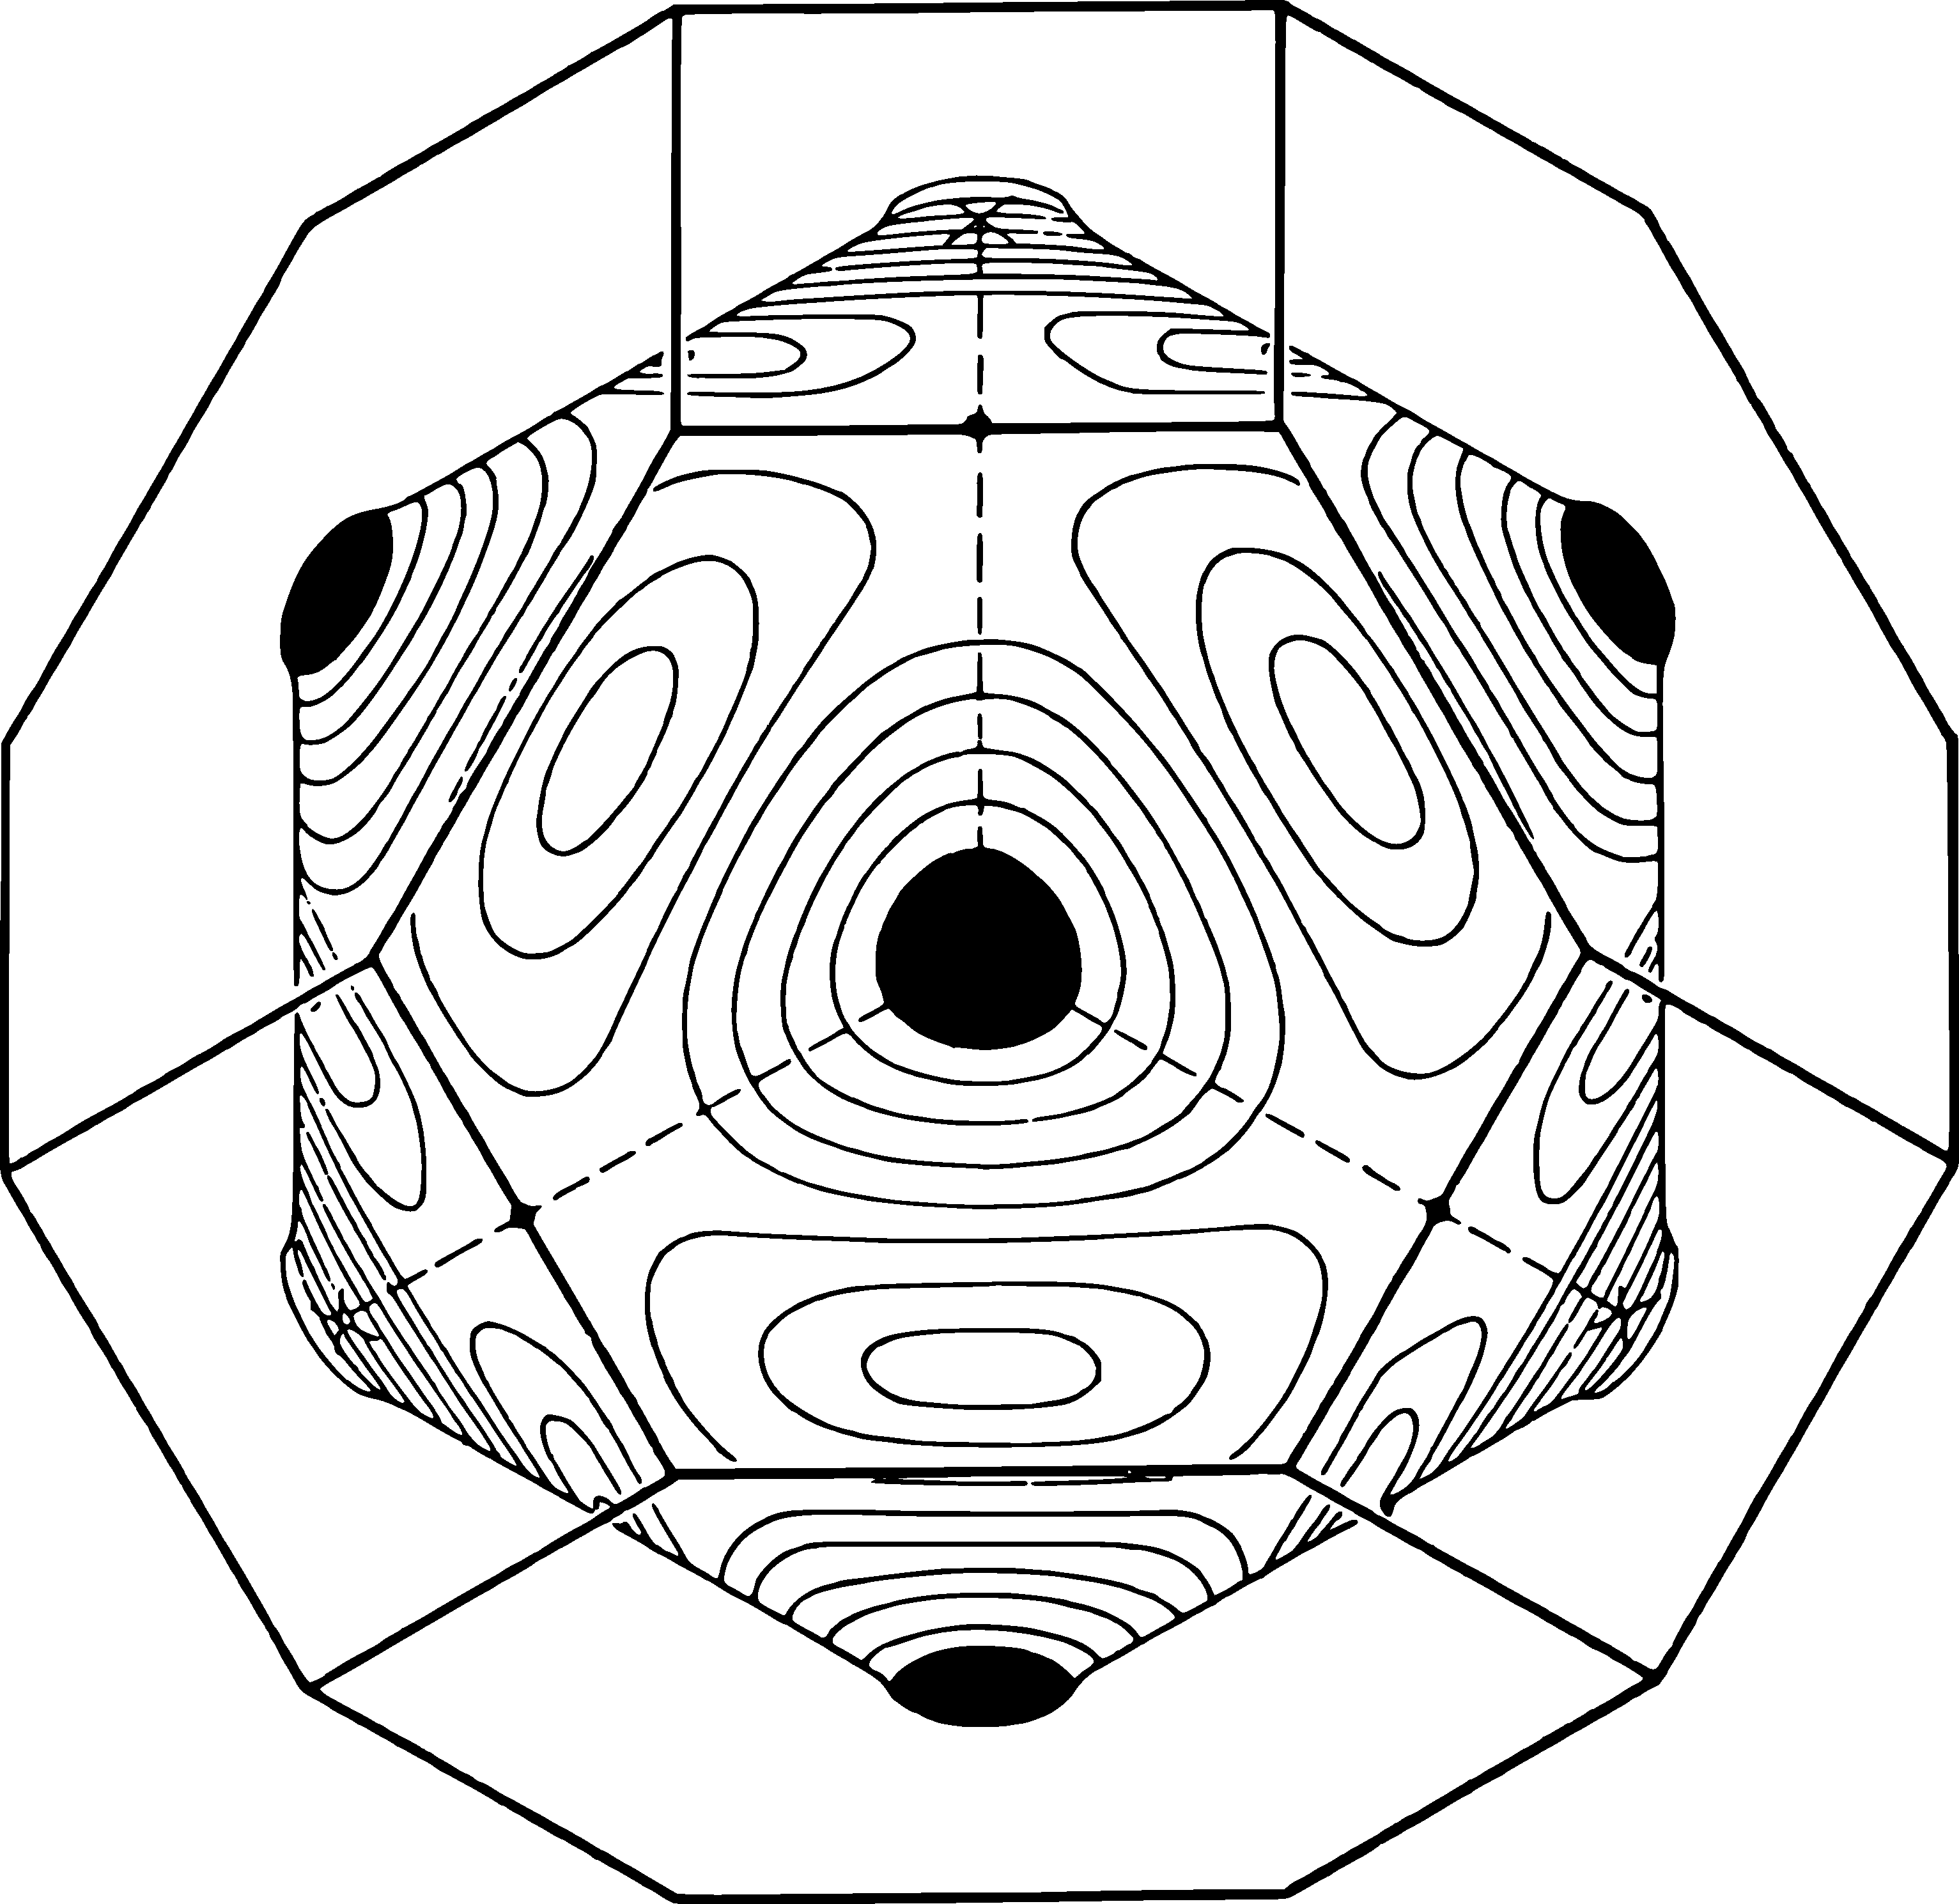
\includegraphics[width=0.45\textwidth]{graphics/fermi_copper_pippard}%
\caption[Isosurface von Kupfer nach Pippard]{Isosurface von Kupfer nach Pippard \cite{Pippard1957}}%
\label{fig:fermi_copper_pippard}%
\end{figure}